\documentclass{scrartcl}
\usepackage[utf8]{inputenc}
\usepackage{amsmath}
\usepackage{natbib}
\usepackage{graphicx}
\usepackage{xfrac}


\begin{document}

\section*{Übungsblatt 1 -- Cerberus}

    \subsection*{Aufgabe 1}

        \subsubsection*{a)}

            Bei den hier vorliegenden Gittervektoren handelt es sich um eine hexagonale einatomige Gitterstruktur.

        \subsubsection*{b)}

            Es soll nun folgendes Gleichungssystem \(\mathbf{A} \vec{x} = \vec{b}\) mithilfe der LU-Zerlegung gelöst werden:
            \begin{equation*}
                \begin{pmatrix}
                    \sfrac{1}{2} & -\sfrac{1}{2} & 0 \\
                    \sfrac{\sqrt{3}}{2} & \sfrac{\sqrt{3}}{2} & 0 \\
                    0 & 0 & 1 
                \end{pmatrix}
                \cdot \vec{x} =
                \begin{pmatrix}
                    2 \\ 
                    0 \\ 
                    2 
                \end{pmatrix}.
            \end{equation*}
            Die $\mathbf{P}$-, $\mathbf{L}$- und $\mathbf{U}$-Matrizen werden mit \verb|Eigen::PartialPivLU| aus der Eigen-Bibliothek bestimmt und lauten:
            \[
                \mathbf{P} = 
                \begin{pmatrix}
                    0 & 1 & 0 \\
                    1 & 0 & 0 \\
                    0 & 0 & 1 
                \end{pmatrix}
                \quad
                \mathbf{L} =
                \begin{pmatrix}
                    1 & 0 & 0 \\
                    0.57735 & 1 & 0 \\
                    0 & 0 & 1 
                \end{pmatrix},
                \quad
                \mathbf{U} = 
                \begin{pmatrix}
                    0.866025 & 0.866025 & 0 \\
                    0 & -1 & 0 \\
                    0 & 0 & 1 
                \end{pmatrix},
            \]
            Nun lässt sich $\mathbf{A} \vec{x} = \vec{b}$ als $\mathbf{P} (\mathbf{L} (\mathbf{U} \vec{x})) = \vec{b}$ schreiben, 
            wobei
            \begin{align}
                \mathbf{P} \vec{z} &= \vec{b} \label{eqn:1} \\
                \mathbf{L} \vec{y} &= \vec{z} \label{eqn:2} \\
                \mathbf{U} \vec{x} &= \vec{y} \label{eqn:3}
            \end{align}
            gilt. Gleichung \eqref{eqn:1} wird durch
            \[ 
                \vec{z} = \mathbf{P}^{\text{T}} \vec{b}
            \]
            gelöst. Die Lösung von Gleichung \eqref{eqn:2} erfolgt rekursiv über
            \begin{align*}
                y_1 &= \frac{z_1}{L_{11}} \\
                y_i &= \frac{1}{L_{ii}} \left(z_i - \sum_{j=1}^{i-1} L_{ii} y_i \right).
            \end{align*}
            Gleichung \eqref{eqn:3} wird ähnlich wie Gleichung \eqref{eqn:2} gelöst, wobei die Elemente aber absteigend angefangen
            mit dem letzten Element $x_\text{n}$ berechnet werden
            \begin{align*}
                x_{\text{n}} &= \frac{y_{n}}{U_{nn}} \\
                x_i &= \frac{1}{U_{ii}} \left(y_i - \sum_{j=i+1}^{n} U_{ij} x_i \right).
            \end{align*}
            Der Ergebnisvektor lautet schließlich
            \begin{equation*}
                \vec{x} = 
                \begin{pmatrix}
                    2 \\
                    -2 \\
                    2   
                \end{pmatrix}.
            \end{equation*}

        \subsubsection*{c)}

            Da sich die Basis nicht ändert, kann die mit Eigen berechnetet LU-Zerlegung, die einen Aufwand von $\mathcal{O} (N^3)$ hat, 
            weiterverwendet werden und es muss nur noch
            die Berechnung von Gleichung \eqref{eqn:1} bis \eqref{eqn:3} erfolgen. Diese enthalten jeweils $\mathcal{O}(N^2)$ Operationen.
            Der Ergebnisvektor lautet
            \begin{equation*}
                \vec{x} = 
                \begin{pmatrix}
                    3 \\
                    1 \\
                    1   
                \end{pmatrix}.
            \end{equation*}

        \subsubsection*{d)}

            Die LU-Zerlegung für die neue Basis 
            \[
                \mathbf{A} =
                \begin{pmatrix}
                    0 & -\sfrac{1}{2} & \sfrac{1}{2} \\
                    0 & \sfrac{\sqrt{3}}{2} & \sfrac{\sqrt{3}}{2} \\
                    1 & 0 & 0 \\
                \end{pmatrix}
            \]
            lautet 
            \begin{align*}
                \mathbf{P} = 
               \begin{pmatrix}
                   0 & 0 & 1 \\
                   0 & 1 & 0 \\
                   1 & 0 & 0 
               \end{pmatrix}
               \quad
               \mathbf{L} =
               \begin{pmatrix}
                   1 & 0 & 0 \\
                   0 & 1 & 0 \\
                   0 & -0.57735 & 1 
               \end{pmatrix},
               \quad
               \mathbf{U} = 
               \begin{pmatrix}
                   1 & 0 & 0 \\
                   0 & 0.866025 & 0.866025 \\
                   0 & 0 & 1 
               \end{pmatrix}.
            \end{align*}
            Die $\mathbf{L}$- und $\mathbf{U}$-Matrizen unterscheiden sich im Wesentlichen durch durch je eine zyklische Vertauschung der Zeilen und der Spalten, 
            während sich die $\mathbf{P}$-Matrizen nur durch eine zyklische Vertauschung der Zeilen unterscheiden.

        \subsubsection*{e)}

            Wenn die primitiven Gittervektoren paarweise orthogonal sind ist $\mathbf{A}$ regulär und es gilt $\mathbf{A}^{-1} = \mathbf{A}^{\text{T}}$.

\newpage
\subsection*{Aufgabe 2}
Für den Datensatz
\begin{table}[]
    \centering
\label{tab:data_tab}
	\sisetup{table-format=1.2}
	\begin{tabular}{S[table-format=2.1]S[table-format=2.1]}
		\toprule
		{$x$} & {$y$} \\
		\midrule
		0.0 & 4.0 \\
		2.5 & 4.3 \\
		-6.3 & -3.9 \\
		4.0 & 6.5 \\
		-3.2 & 0.7 \\
		5.3 & 8.6 \\
		10.1 & 13.0 \\
		9.5 & 9.9 \\
		-5.4 & -3.6 \\
		12.7 & 15.1 \\
		\bottomrule
	\end{tabular}

\end{table}
soll eine lineare Regression der Form
\[
y = mx + n
\]
durchgeführt werden, die den quadratischen Fehler minimiert.\\
Zunächst lässt sich das lineare Gleichungssystem $A\vec{x}=\vec{b}$ aufstellen als
\[
\begin{pmatrix}
   0  & 1\\
 2.5  & 1\\
-6.3  & 1\\
   4  & 1\\ 
-3.2  & 1\\
 5.3  & 1\\
10.1  & 1\\
 9.5  & 1\\
-5.4  & 1\\
12.7  & 1
\end{pmatrix}\cdot
\begin{pmatrix}
m\\
n
\end{pmatrix} = 
\begin{pmatrix}
4\\
4.3\\
-3.9\\
6.5\\
0.7\\
8.6\\
13\\
9.9\\
-3.6\\
15.1
\end{pmatrix}
\]
Durch multiplizieren mit der Transponierten der Matrix $A$ wird wandelt sich das
System zu $A^TA\vec{x} = A^T \vec{b} = \vec{b}'$, mit der quadratischen Matrix
\[
A^TA = \begin{pmatrix}
482.98 & 29.2 \\
  29.2  &  10 
\end{pmatrix}
\]
und dem neuen Ergebnisvektor
\[
\vec{b}' = \begin{pmatrix}
541.22\\
  54.6
\end{pmatrix}\text{.}
\]
Eine numerische LU-Zerlegung $A^TA = PLU$ liefert die Pivotisierungs-Matrix
\[
P = 
\begin{pmatrix}
1 & 0\\
0 & 1
\end{pmatrix},
\]
die L-Matrix
\[
L = \begin{pmatrix}
       1    &   0\\
0.060458    &   1
\end{pmatrix}
\]
und die U-Matrix
\[
U = \begin{pmatrix}
 482.98 &  29.2\\
      0 & 8.23463
\end{pmatrix}.
\]
Damit ergibt sich die Lösung für die lineare Regression zu
\[
y = 0.959951\cdot x + 2.65694\; .
\]
In Abbildung \ref{fig:linreg} ist diese Ausgleichsgerade und die zugehörigen Daten zu sehen.
\begin{figure}
    \centering
    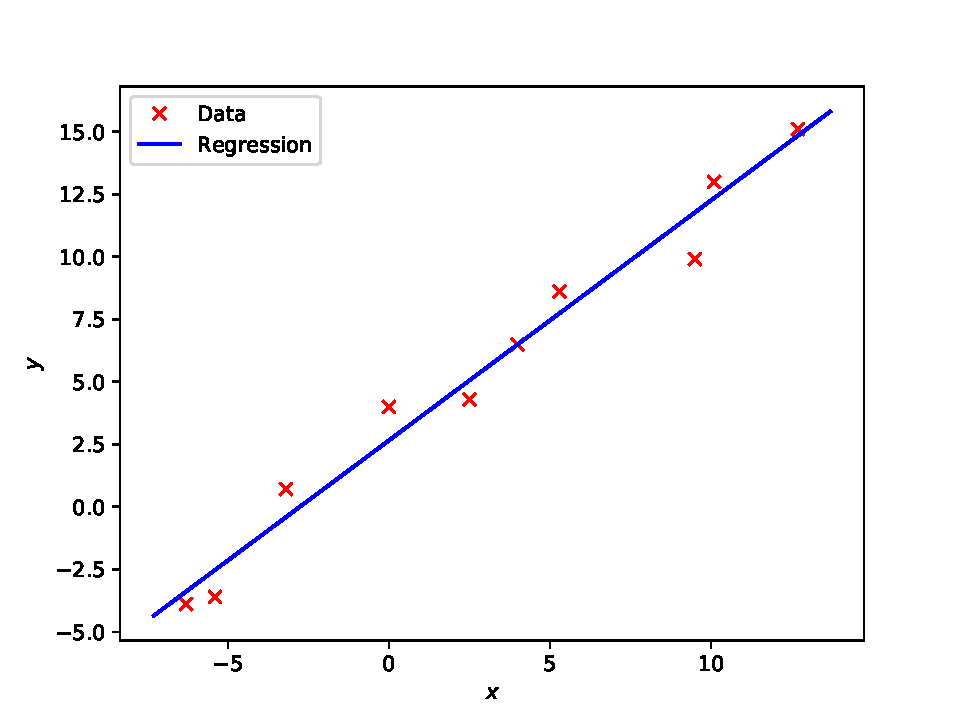
\includegraphics[width=\textwidth]{A2/build/Regression.pdf}
    \caption{Lineare Regression zum Datensatz\ref{tab:data_tab}.}
    \label{fig:linreg}
\end{figure}

\end{document}
